\documentclass{article}
\usepackage{cmap}
\usepackage[T2A]{fontenc}
\usepackage[utf8]{inputenc}
\usepackage[english,russian]{babel}
\usepackage{setspace}
\usepackage{geometry}
\usepackage{graphicx}
\usepackage{amsfonts}
\usepackage{amsmath}
\graphicspath{{graphicslab5/}}
\DeclareGraphicsExtensions{.pdf, .png, .jpg, .fig}
\geometry{top=2cm}
\geometry{bottom=2cm}
\geometry{left=2cm} % отступ справа
\geometry{right=2cm} % отступ слева

\begin{document}
	\begin{center}
		\hfill \break
		\begin{center}
			\huge{Санкт-Петербургский политехнический университет\\
				Высшая школа прикладной математики\\
				и вычислительной физики, ФизМех}
		\end{center}
		\hfill \break
		\hfill \break
		\hfill \break
		\hfill \break
		\hfill \break
		\huge{Направление подготовки\\
			«Прикладная математика и информатика»}\\
		\hfill \break
		\hfill \break
		\hfill \break
		\hfill \break
		\hfill \break
		\hfill \break
		\fontsize{14pt}{14pt}\selectfont
		Отчет по лабораторной работе №5\\
		«Численнные методы решения задачи Коши для обыкновенных дифференциальных уравнений»\\
		\hfill \break
		\hfill \break
		\hfill \break
		\hfill \break
		\hfill \break
	\end{center}
	\hfill \break
	\hfill \break
	\fontsize{12pt}{12pt}\selectfont
	\begin{tabular}{cccc}
		\hspace{1cm}Выполнил студент гр. 5030102/00003 & {\hspace{3cm}} & & Петрошенко А.В. \\\\
		\hspace{-3cm}Преподаватель: &{\hspace{1cm}}& & {\hspace{1cm}} Курц В.В. \\\\
	\end{tabular}\\
	\hfill \break
	\hfill \break
	\hfill \break
	\hfill \break
	\hfill \break
	\hfill \break
	\begin{center} Санкт-Петербург\\ 
		2021\\
	\end{center}
	\thispagestyle{empty}
	\newpage
	\begin{center} \textbf{Формулировка задачи и ее формализация}\end{center}
	\underline{Постановка задачи:}\\
	Дифференциальное уравнениеn­го порядка
	\begin{equation}
		F(x, y, y', ..., y^{(n)}) = 0
	\end{equation}
	где $y(x)$ - неизвестная функция\\
	Уравнение (1), разрешенное относительно старшей производной
	\begin{equation}
		y^{(n)} = f(x, y, y', ..., y^{(n-1)})
	\end{equation}
	Общее решение: $y(x) = y(c_1, ..., c_n)$ - $n$-параметрическое семейство\\
	Пусть через любую точку проходит единственная интегральная кривая. Чтобы выделить единственное решение, нужно задать $n$ условий.\\
	\\
	В данной лабораторной работе будут решаться уравнения 1-го и 2-го порядков\\
	Пусть задача решается на конечном отрезке $[a,b]$ и все условия заданы в одной точке $[a,b] \rightarrow$ задача Коши, или задача с начальными условиями.
	\begin{center} \textbf{Алгоритм метода и условия его применимости}\end{center}
	\underline{Метод Рунге-Кутты 3-го порядка с коэффициэнтом 1/2}\\
	Задача Коши
	\begin{equation}
		\begin{cases}
			y' = f(x, y)\\
			y(a) = y_0
		\end{cases}	
	\end{equation}
	$x, x+h \in [a, b]$
	\begin{equation}
		y(x+h) = y(x) + \underbrace{\frac{h}{1!} y'(x) + \frac{h^2}{2!} y''(x) + ... + \frac{h^s}{s!} y^{(s)}(x)}_{\Delta_sy(x)} + O(h^{s+1})
	\end{equation}
	Заменим $\Delta_sy(x)$ некоторой функцией $\delta_sy(x,h)$, которая удовлетворяет условию
	\begin{equation}
		\Delta_sy(x) = \delta_sy(x,h) + O(h^{s+1}) 
	\end{equation}
	Будем искать $\delta_sy(x,h)$ в виде линейной комбинации значений $f$
	\begin{equation}
		\displaystyle \delta_sy(x,h) = h\sum_{i=1}^{l}\rho_if(x + \delta x_i, y + \delta y_i) 
	\end{equation}
	где $s$ - порядок метода, $l$ - шаговость или стадийность метода
	Подберем $l$, $\rho_i$, $\delta x_i$ и $\delta y_i$ так, чтобы (5) выполнялось.
	Выбираем $l$. Будем искать $\delta_sy(x,h)$ в виде:
	\begin{equation}
		\displaystyle \delta^l_sy(x,h) = h\sum_{i=1}^{l}\rho_iK_i
	\end{equation}
	где 
	\begin{equation}
		\begin{cases}
			K_1 = f(x,y)\\
			K_2 = f(x + \alpha_2h,y + h\beta_{21}K_1)\\
			K_3 = f(x + \alpha_3h,y + h\beta_{31}K_1 + h\beta_{32}K_2)\\
			...\\
			\displaystyle K_l = f(x + \alpha_lh, y + h\sum_{j=1}^{l-1}\beta_{lj}K_j)
		\end{cases}	
	\end{equation}
	Коэффициенты $\rho_i$, $\alpha_i$, $\beta_{ij}$ выбираются из условия (5): обеспечение порядка апроксимации $s$.
	Тогда в (4) отбросим $O(h^{s+1})$, $x \rightarrow x_k$, $x+h \rightarrow x_k+1$
	\begin{equation}
		y_{k+1} = y_k + h\sum_{i=1}^{l}\rho_iK_i
	\end{equation}
	\underline{Алгоритм метода}\\
	\begin{equation}
		\begin{cases}
			y_{i+1} = y_i + \frac{h}{6}(K_1 + 4K_2 + K_3)\\
			K_1 = f(x_i, y_i)\\
			K_2 = f(x_i + \frac{h}{2}, y_i + \frac{h}{2}K_1)\\
			K_3 = f(x_i + h, y_i - hK_1 + 2hK_2)
		\end{cases}	
	\end{equation}
	Таким образом в данной работе реализуется 3-х стадийный метод 3-го порядка.\\
	\underline{Условия применимости}
	\begin{enumerate}
		\item Функция $f$ должна быть достаточное число раз непрерывно дифференцируемой.
		\item $x+h \in [a,b]$
	\end{enumerate}
	\begin{center} \textbf{Предварительный анализ задачи}\end{center}
	Мы строим равномерную сетку для $[a,b]$, поэтому  2-ой пункт выполнен по построению\\
	\\
	В данной работе будет рассматриваться ОДУ $xy' + (x+1)y = 3x^2e^{-x}$, значит $\displaystyle f = \frac{3x^2e^{-x} - (x+1)y}{x}$, которая бесконечно дифференцируема.
	\begin{center} \textbf{Тестовый пример для задач малой размерности}\end{center}
	$\displaystyle f(x,y) = \frac{3x^2e^{-x} - (x+1)y}{x}$, точное решение $y^*(x) = x^2e^{-x}$\\
	Начальное условие на $[a,b]$ $y(a) = 1/e$, где $a = 1$, $b = 5$\\ 
	Возьмем $\displaystyle h = \frac{b-a}{2} = 2$ и сделаем 2 шага по $h$, 1 шаг $2h$ и оценим погрешность с помощью правила Рунге.\\
	$$\epsilon^{(h)}_{k+2} \approx \frac{y^{(2h)}_{k+2} - y^{(h)}_{k+2}}{2^s - 1} $$
	\underline{1 Шаг}\\
	\begin{equation}
		\begin{cases}
			y_b = y_a + \frac{2}{3}(K_1 + 4K_2 + K_3)\\
			K_1 = f(x_a, y_a)\\
			K_2 = f(x_a + 2, y_a + 2K_1)\\
			K_3 = f(x_a + 4, y_a - 4K_1 + 8K_2)
		\end{cases}	
	\end{equation}
	$$K_1 = 0.368$$
	$$K_2 = -1.024$$
	$$K_3 = 11.256$$
	$$y_b = 5.386$$
	Фактическая погрешность: $|y^*(b) - y_b| = 5.386 - 0.168 = 5.218$\\
	\underline{2 Шага}\\
	\begin{equation}
		\begin{cases}
			y_{(b-a)/2} = y_a + \frac{2}{3}(K_1 + 4K_2 + K_3)\\
			K_1 = f(x_a, y_a)\\
			K_2 = f(x_a + 2, y_a + 2K_1)\\
			K_3 = f(x_a + 4, y_a - 4K_1 + 8K_2)
		\end{cases}	
	\end{equation}
	$$K_1 = 0.368$$
	$$K_2 = -0.292$$
	$$K_3 = 2.494$$
	$$y_{(b-a)/2} = 0.933$$
	\begin{equation}
		\begin{cases}
			y_b = y_{(b-a)/2} + \frac{2}{3}(K_1 + 4K_2 + K_3)\\
			K_1 = f(x_{(b-a)/2}, y_{(b-a)/2})\\
			K_2 = f(x_{(b-a)/2} + 2, y_{(b-a)/2} + 2K_1)\\
			K_3 = f(x_{(b-a)/2} + 4, y_{(b-a)/2} - 4K_1 + 8K_2)
		\end{cases}	
	\end{equation}
	$$K_1 = -0.796$$
	$$K_2 = 0.048$$
	$$K_3 = -3.161$$
	$$y_b = -0.321$$
	Фактическая погрешность: $|y^*(b) - y_b| = 0.168 + 0.321 = 0.489$\\
	Правило Рунге: $\displaystyle \epsilon^{(h)}_{k+2} \approx \frac{y^{(2h)}_{k+2} - y^{(h)}_{k+2}}{2^s - 1} = \frac{5.386 + 0.321}{7} = 0.815$\\
	Фактическая погрешность и погрешнсть по правилу Рунге одного порядка, но погрешность по Рунге больше.
	\begin{center} \textbf{Контрольные тесты}\end{center}
	\begin{enumerate}
		\item Разобъем отрезок $[a,b]$ на $2^5$ частей и решим ур-ние нашим методом
		\item Будем разбивать наш отрезок на части(от 1 до $2^{15}$) и посмотрим на зависимость локальной и глобальной погрешностей
		\item Зададим возмущение(порядка от $10^{-10}$ до $10^0$) в начальное условие и посмотрим, как меняется погрешность при шаге $1/2^{10}$
	\end{enumerate}
	\begin{center} \textbf{Модульная структура программы}\end{center}
	\verb|double f(double x, double y)|\\
	\verb|double y(double x)|\\
	-Функция $f$ и функция точного решения $y = e^{-x}$\\
	\verb|double Calculate(double h, double x_j, double y_j)|\\
	-Функция для вычисления значения $y$ на следующем шаге\\
	\verb|void Error(double a, double f_a, double b, ofstream* F)|\\
	-Функция для вычисления локальной и глобальной погреностей\\
	\verb|vector<double> Runge_Kutta(double a, double f_a, double b, int n)|\\
	-Функция решения ОДУ\\
	\verb|double Pertubation(double a, double f_a, double df_a, double b, int n)|\\
	-Функция решения ОДУ с возмущением
	\newpage
	\begin{center} \textbf{Численный анализ}\end{center}
	$\triangleright$ \underline{Точное и численное решение:}\
	\begin{center} 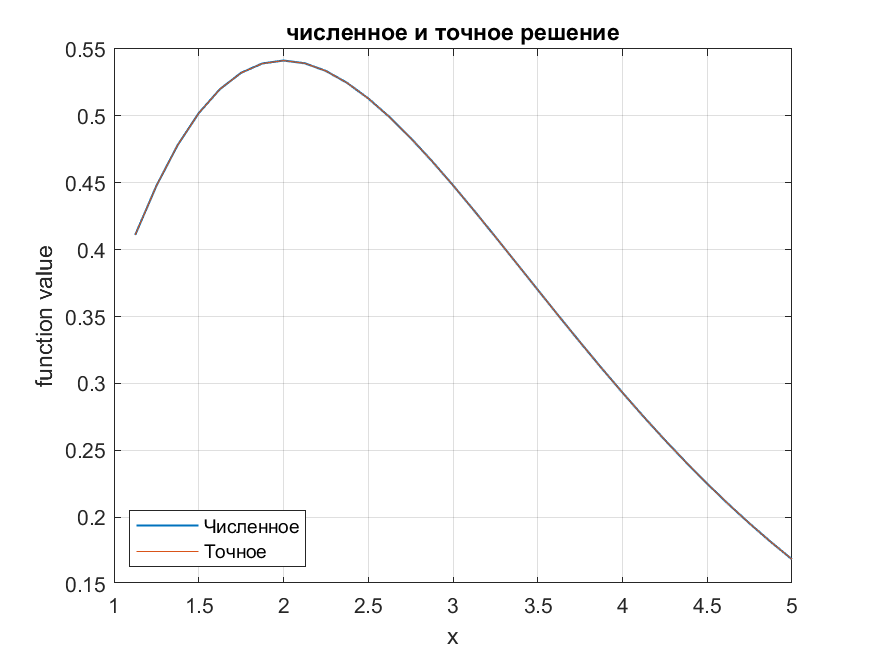
\includegraphics[scale = 0.6]{решение} \end{center}
	Оба графика накладываются друг на друга, что показывает, что решения практически совпадают.\\
	$\triangleright$ \underline{Ошибка численного решения:}
	\begin{center} 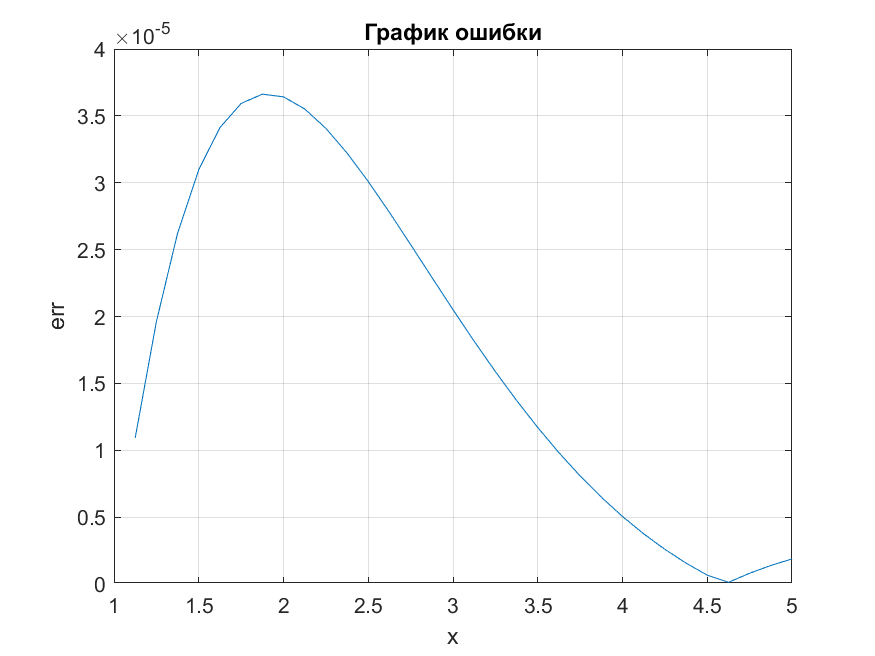
\includegraphics[scale = 0.6]{ошибка} \end{center}
	В начальной точке ошибка очевидно нулевая, т.к. мы просто подставили начальное условие. Ошибка ненулевая, порядка $10^-5$. На конце происходит небольшой излом, что обуславливается видом интегральной кривой. В какой то момент мы просто перешагнули через нужную кривую и ошибка снова возросла.\\
	$\triangleright$ \underline{Погрешности:}
	\begin{center} 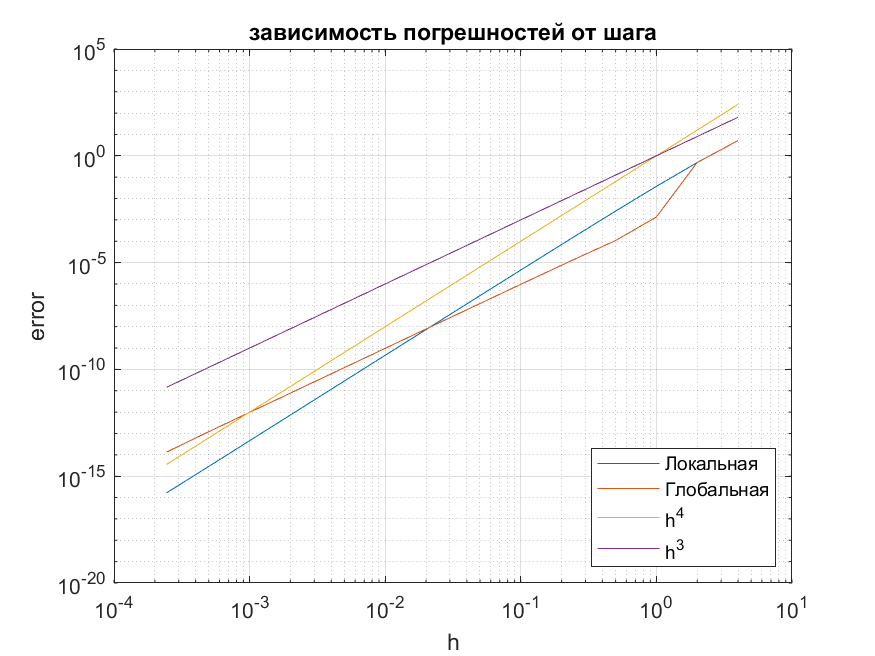
\includegraphics[scale = 0.6]{погрешность} \end{center}
	Порядки погрешностей совпадают с установленными методом порядками, что означает, что метод реализован правильно. Погрешности пересекаются, что так же обуславливается видом интегральной кривой.\\
	$\triangleright$ \underline{Возмущение:}
	\begin{center} 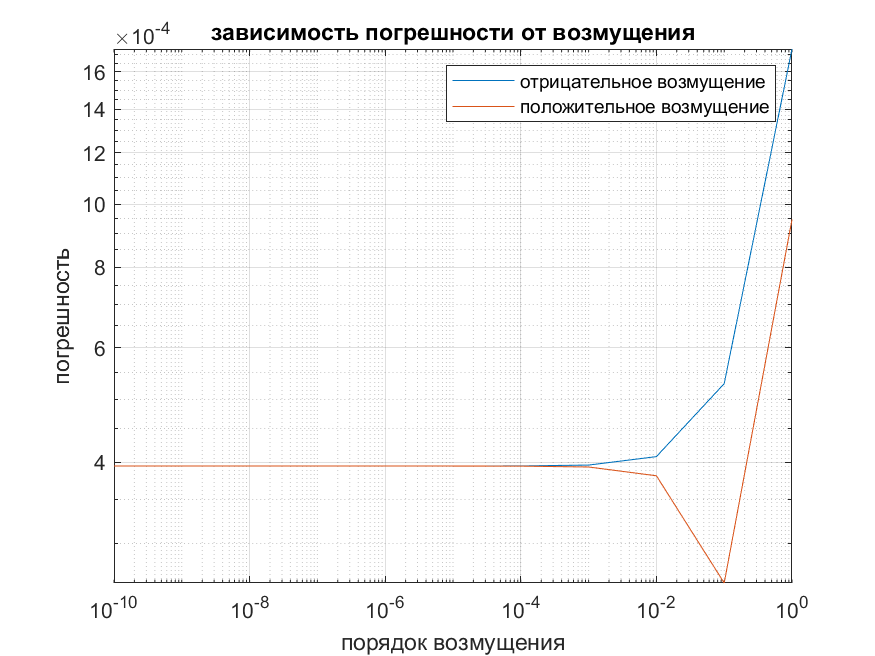
\includegraphics[scale = 0.6]{возмущение} \end{center}
	Мы рассмотрели 2 возмущения: отрицательное и положительное. При малых возмущениях погрешность не меняется, но начиная с $10^{-3}$ они отклоняются, что совпадает с порядком погрешности метода. При чем одна уменьшается, а другая увеличивается, для разных кривых это отклонение будет разным, но для достаточно больших возмущений обе погрешности увеличиваются.
	\begin{center} \textbf{Общие выводы}\end{center}
	В данной лабораторной работе мы научились численно решать ОДУ 1-го и 2-го порядка на заданном промежутке с помощью метода Рунге-Кутты 3-го порядка с коэффициентом 1/2. Реализация метода очень простая, что видно из модульной структуры. Метод довольно эффективный, но он, как и все остальные, зависит от вида интегральной кривой.
\end{document}